\documentclass[11pt]{article}
\usepackage[UTF8]{ctex}
\usepackage{indentfirst}
%\setlength{\parindent}{2em}

% some package

% graph
\RequirePackage{graphicx}
\RequirePackage{subfigure}
\RequirePackage{float}
% math
\RequirePackage{amsmath}
\RequirePackage{amssymb,amsfonts,mathrsfs}

\RequirePackage{bm}         % \mathbf{}
\RequirePackage{color}      % the color of the font
\usepackage{mathrsfs}
\RequirePackage{enumerate}

% like word
\usepackage[top=2.54cm, bottom=2.54cm, left=3.17cm, right=3.17cm]{geometry}


%\usefonttheme{professionalfonts}

% the caption of thf figure
\renewcommand{\figurename}{图}


\title{ \textbf{生物智能课程论文-知识图谱} }


\author{
	张永辉  \qquad 计算机学院  \qquad 21721042\\
	21721042@zju.edu.cn
}

\date{ }

\begin{document}
	
	\maketitle
	\section{什么是知识图谱}
	随着计算机技术发展,人们对计算机的检索查询能力要求越来越高。人们希望能有一个能为用户提供加工和推理过的知识的查询环境。而知识图谱(Knowledge Graph)则是实现智能化语义检索的基础和桥梁\cite{Liu2016}。传统搜索引擎技术能够根据用户查询快速排序网页,提高信息检索效率。然而,这种网页检索的高效率并不等同用户能够准确快速的获取信息和知识。对于搜索引擎返回的结果,用户还需要进行人工的筛选和排序。当前互联网上的信息呈爆炸式发展,这样的检索方式很难满足人们全面掌控信息资源的需求。同时,有些问题的答案虽然已经明确存在,但是由于其包含了太多的限定和逻辑,以至于互联网上也很难存在完全一样的信息。知识图谱技术的出现为解决信息检索问题提供了新的思路。

	知识图谱的概念是由谷歌公司提出的,2010年Google收购了Metaweb公司并获得了该公司的语义搜索技术,其中的关键技术包括从互联网网页中抽取出实体及其属性信息,和实体之间的关系信息。这些技术特别适合与实体相关的智能问答问题,由此创造出一种全新的信息检索模式。
	
	\subsection{知识图谱的定义}
	知识图谱是结构化的语义知识库,用于以符号形式描述描述现实世界中的实体及其之间的相互关系。其基本组成是\textbf{实体-关系-实体}三元组,以及实体和其相关属性的值对,实体之间通过关系相互连接,构成网状的知识结构。\cite{Liu2016}
	
	通过知识图谱,可以实现Web从网页链接到概念链接的转变,支持用户按主题而不是字符串进行检索基于知识图谱的搜索引擎,能够向用户返回结构化的知识,用户不必自行浏览大量网页,就可以准确有深度的获取知识。
	
	知识图谱的定义包含有三层含义
	
	\begin{enumerate}
		\item 知识图谱本身是一个具有属性的实体通过关系链接而成的网状结构的知识库。从图的角度来看,知识图谱其实是一个概念网络。其中的节点表示真实世界中的实体,而边表示实体之间的各种语义关系。所以说知识图谱是对真实世界的一种符号表达
		\item 知识图谱的研究价值在于,知识图谱是构建在当前Web之上的一层覆盖网络,借助知识图谱,能够在Web网页之间建立概念之间的联系关系,从而将互联网中积累的信息组织起来,成为可以被利用的知识。
		\item 知识图谱的应用价值在于,她能够改变现有的信息检索方式。一方面,区别于大部分现在基于字符串的检索方式,知识图谱能够实现基于推理实现概念搜索。另一方面,知识图谱可以向用户展示经过分类整理的结构化知识,从而将用户从人工过滤网页阅读寻找答案的模式中解放出来。
	\end{enumerate}

	\subsection{知识图谱的结构}
	从逻辑上讲,知识图谱可划分为两个层次,数据层和模式层。在知识图谱的数据层,知识以事实为单位存储在图数据库中。例如Google Graphd 和 Microsoft Trinity 都是典型的图数据库。如果以实体-关系-实体或者实体-属性-值三元组作为事实的基本表达方式,则存储在图数据库中的所有数据将构成庞大的实体关系网络,形成知识的“图谱”。
	模式层在数据层之上,是知识图谱技术的核心,在模式层存储的经过提炼的知识,通常采用本体数据库来管理知识图谱的模式层。借助本体库对公理,规则和约束条件的支持能力来规范实体、关系和实体类型和属性等对象之间的联系。本体库在知识图谱中的地位相当于知识库的模具,拥有本体库的知识库冗余知识较少。
		
		
	\section{知识图谱的构建}
	图\ref{figure01}给出了知识图谱技术的整体架构,其中许仙内的部分为知识图谱构建的过程,也是知识图谱的更新过程。如图所示,知识图谱的构建过程是从原始数据出发,采用一系列自动或者半自动的技术手段,从原始
	数据中提取出只是要素,或者说提取出事实,并将其存入知识库的数据层和模式层的过程。这是一个迭代更新的过程,根据知识获取的逻辑,每一轮迭代包含三个阶段:\textbf{信息抽取},\textbf{知识融合}和\textbf{知识加工}
	
	知识图谱头自顶向下和自底向上两种构建方式。所谓自顶向下构建是借助百科类网站等结构化数据源,从高质量数据中题取本体和模式信息,加入到知识库中。所谓自底向上构建,则是借助一定的技术手段,从公开的数据集中提取出模式,选择其中之心度较高的模式,经过人工审核后,加入到知识库中去。
	
	
	\begin{figure}[htbp]
		\centering
		%\flushleft
		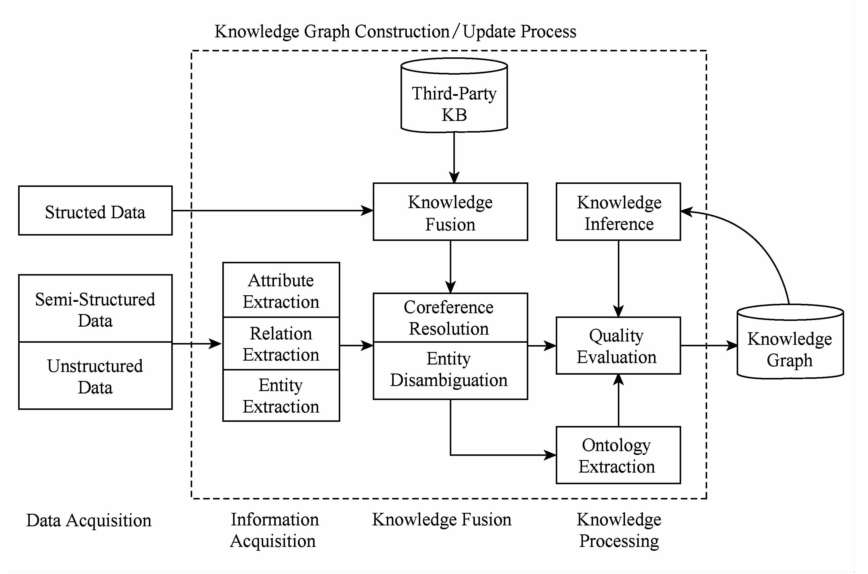
\includegraphics[width=0.7\textwidth]{pic/build_kg.png}
		\caption{知识图谱架构}
		\label{figure01}
	\end{figure}
	\subsection{信息抽取}
	信息抽取主要分为实体抽取,关系抽取和属性抽取三部分。
	
	实体抽取也称为命名实体识别(named entity recgnition, NER),指从文本数据集中自动识别出命名实体。实体的抽取质量(准确率和召回率)对后取得知识获取效率和质量影响极大,因此是信息抽取中最为基础和关键的部分。
	
	文本语料经过实体抽取,得到的是一系列离散的命名实体,为了得到语义信息,还需从相关语料中提取出实体之间的关系联系,通过关系将实体联系起来才能够形成网状的知识结构。
	
	早期关系抽取主要是通过人工构造语法和语义规则,据此采用模式匹配的方法来识别实体间的关系。这种方法有两点明显不足:第一,要求制定规则的人具有良好而语言学造诣,并且对特定领域有深入理解和认知;第二,规则制定工作量大,难以适应丰富的语言表达风格,且难以拓展到其他领域。之后,学术界开始尝试采用统计机器学习方法,通过对实体间关系的模式进行建模,替代预定义的语义和语法规则。
	
	属性抽取的目标是从不同的信息源中采集特定的实体的属性信息,例如针对某个公众人物,可以从网络公开信息中获得其昵称、生日、教育背景和国际等信息。属性抽取技术能够从多种数据来源中汇集这些信息,实现对实体属性的完整勾画。
	
	\subsection{知识融合}
	通过信息抽取,实现了从非结构化数据和半结构化数据中获取实体,关系以及实体属性信息的目标,然而,这些结果中可能包含大量冗余和错误信息,数据之间的关系也是扁平化的,缺乏层次性和逻辑性,一次有必要对其进行清理和整合。知识融合包括两部分内容,\textbf{实体链接}和\textbf{知识合并},通过知识融合,可以消除歧义概念,剔除冗余和错误概念,从而确保知识的质量。
	
	实体链接(entity linking)是指对于从文本中抽取得到实体对象,将其连接到知识库中对应正确实体对象的操作。
	
	实体链接的基本思想是首先根据给定的实体指称项,从知识库中选出一组候选的实体对象。实体链接的基本流程是:首先从文本中通过实体抽取得到实体指称项;然后进行消歧义和共指消解,判断知识库中同名实体是否代表不同含义,以及知识库是否存在命名实体与其他命名实体表示相同含义;最后确认知识库中对应的正确实体对象后,将实体指称项连接到知识库中的对应实体。
	
	\subsection{知识加工}
	通过信息学抽取,剋从原始语料中提取出实体,关系与属性等知识要素,再经过知识融合,可以消除实体指称项与实体对象之间的歧义,得到一系列基本的事实的表达。然而事实并不等于知识,要想最终获得结构化网格化的知识体系,还需要知识加工。知识加工主要包括三方面:本体构建,知识推理和质量评估。
	
	本体(ontology)是对概念进行建模的规范,是描述客观世界的抽象规范,以形式化的方式对概念及其之间的联系给出明确的定义,本体的最大特点在于它是共享的,本体中反映的知识是一种明确定义的共识。本体是一种树状结构,这种单纯的关系有助于知识推理,但却不利于表达概念的多样性,在知识图谱中,本体位于模式层。
	
	本体可以由人工编辑的方式手动创建,也可以由计算机辅助,以数据驱动的方式自动构建,然后采用算法评估和人工审核的方式加以修正和确认。
	
	知识推理是指从知识库中与有的实体关系数据出发,经过计算机推理,建立实体间的新关联,从而拓展和丰富知识网络。知识推理是知识图谱构建的重要环节和手段。通过只是推理,可以从现有知识中发现新的知识。
	
	质量评估是知识库构建的重要组成部分,受现有技术水平的限制,采用开放域信息抽取技术得到的知识元素有可能存在错误,经过只是推理得到的知识的质量同样是没有保障的。因此在知识加入知识库前,需要一个质量评估的过程。随着开放关联数据项目的推进,各子项目所产生的知识库产品之间的质量差异也在增大,数据间的冲突也日益增多,。引入质量评估的意义在于,剋对知识的可信度进行量化,通过舍弃置信度较低的知识,可以保证知识库的质量。

	



	
% bibe
\bibliographystyle{plain}
\bibliography{refs}		
\end{document}


